\documentclass[12pt,a4paper]{report}
\usepackage[english]{babel}
\usepackage{newlfont}
\usepackage{color}
\textwidth=450pt\oddsidemargin=0pt
\usepackage[utf8]{inputenc}
\usepackage{fouriernc}
\usepackage[T1]{fontenc}
\usepackage{adjustbox}
\usepackage[margin=2cm]{geometry}
\usepackage{graphicx}
\usepackage{caption}
\usepackage{subcaption}
\usepackage{wrapfig}
\usepackage{tikz}
\usepackage[colorlinks=true,linkcolor=black,urlcolor=black, citecolor=black]{hyperref}
\usepackage{amsmath}
\usepackage{amsthm}
\usepackage{amssymb}
\usepackage{mathtools}
\usepackage{subfiles}
\usepackage{comment}
\usepackage{float}
\usepackage{enumerate}
\usepackage{appendix}
\usepackage[style=numeric, backend=biber, sorting=nty]{biblatex}
\usepackage{chngcntr}
\addbibresource{bibliography.bib}

\setlength{\parindent}{0pt}
\makeatletter
\renewcommand{\fnum@figure}{Fig. \thefigure}
\makeatother


\theoremstyle{plain}
\newtheorem{thm}{Theorem}[section]
\newtheorem{lem}[thm]{Lemma}
\newtheorem{prop}[thm]{Proposition}
\newtheorem{cor}[thm]{Corollary}

\theoremstyle{definition}
\newtheorem{defn}[thm]{Definition}
\newtheorem{exa}[thm]{Example}

\theoremstyle{remark}
\newtheorem{rem}[thm]{Remark}

% \AtAppendix{
%     \renewtheorem{thm}{Theorem}[chapter]
%     \renewtheorem{lem}[thm]{Lemma}
%     \renewtheorem{prop}[thm]{Proposition}
%     \renewtheorem{cor}[thm]{Corollary}
%     \renewtheorem{defn}[thm]{Definition}
%     \renewtheorem{exa}[thm]{Example}
%     \renewtheorem{rem}[thm]{Remark}
% }

%\setcounter{secnumdepth}{0} % no section numbering displayed, no idea how

\newcommand{\bb}[1]{\textbf{#1}}
\newcommand{\ii}[1]{\textit{#1}}
\newcommand{\eps}{\varepsilon}
\newcommand{\N}{\mathbb{N}}
\newcommand{\Z}{\mathbb{Z}}
\newcommand{\R}{\mathbb{R}}
\newcommand{\pder}[2]{\frac{\partial #1}{\partial #2}}
\newcommand{\eval}[1]{\Big{|}_{#1}}
\newcommand{\mc}[1]{\mathcal{#1}}
\newcommand{\mf}[1]{\mathfrak{#1}}
\newcommand{\bmc}[1]{\textbf\mathcal{#1}}
\newcommand{\scal}[2]{\langle #1, #2 \rangle}
\newcommand{\bra}[1]{\langle #1 |}
\newcommand{\ket}[1]{| #1 \rangle}
\newcommand{\braket}[2]{\langle #1 | #2 \rangle}
\newcommand{\del}{\partial}
\newcommand{\then}{\Rightarrow}
\newcommand{\hull}[1]{\langle #1 \rangle}
\newcommand{\m}{\text{-}}
% \newcommand{\ch}[1]{\langle #1 \rangle}
\newcommand{\ch}[1]{\ket{#1}}
% \newcommand{\scal}[2]{#1 \cdot #2 }
\newcommand{\im}{\mathrm{im}\,}
% \newcommand{\ker}{\mathrm{ker}}

\begin{document}
    \begin{titlepage}
        \subfile{sections/front}
    \end{titlepage}
    \pagenumbering{roman}
    %   \subfile{sections/abstract_ita}
    %    \newpage
    %    \subfile{sections/abstract_eng}
    %    \newpage
    \tableofcontents
    \newpage
    \pagenumbering{arabic}
    \begin{chapter}{Preliminaries on topology}
        \label{ch:1}
        The essential idea in algebraic topology is to convert problems about topological spaces and continuous functions into
        problems about algebraic objects and their homomorphisms, this way one hopes to end up with an easier problem to solve. 
        \subfile{sections/1}
    \end{chapter}
    \begin{chapter}{Graphs}
        An important branch of geometric deep learning is graph representation learning. In this section we will therefore
        introduce graphs and graphs laplacians to build a mathematical background for graph neural networks.
        Graphs can be used to encode a wide variety of data, from social networks friendships to maps. An interesting example
        comes from the beginning of topology itself in Koningsberg. Euler noticed that in Koningsberg, there was no path that 
        allowed to cross all seven bridges just once, therefore he started to simplify the problem to approach it in a more mathematical 
        way.
        \begin{figure}[H]
            \begin{minipage}{.5\textwidth}
                \centering
                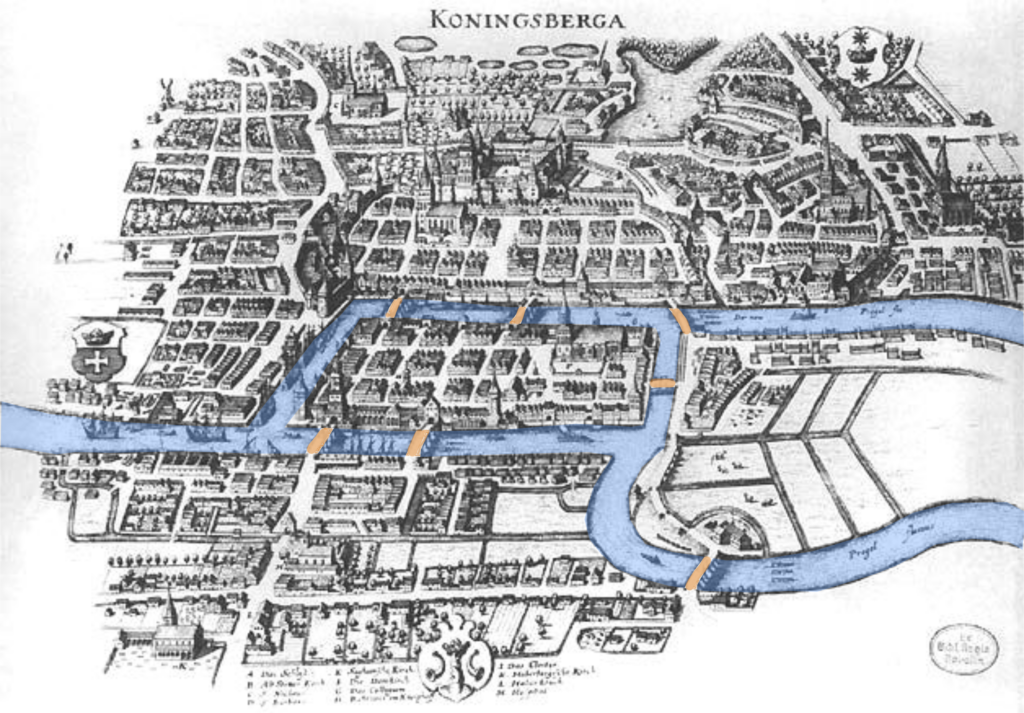
\includegraphics[width=6cm, height=4cm]{sections/2/Bridge}
                \caption{The city of Konigsberg and the\\ seven bridges.}
                \label{fig:2:1}
            \end{minipage}
            \begin{minipage}{.5\textwidth}
                \centering
                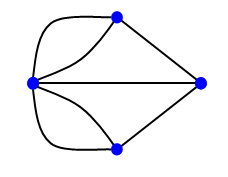
\includegraphics[width=3cm, height=3cm]{sections/2/kgraph}
                \caption{Graph representing Konigsberg's seven bridges}
                \label{fig:2:2}
            \end{minipage}
        \end{figure}
        \subfile{sections/2}
    \end{chapter}
    \begin{chapter}{Geometric Deep Learning}
        \label{ch:3}
        \subfile{sections/3}
    \end{chapter}
    \newpage
   \chapter*{Conclusion}
        Most of the deep learning techniques used today are based on models which learn a partition of the set of smooth functions defined on euclidean 
        domains into human friendly equivalence classes. Although this approach has been successful in modern machine learning, it only deals with a really 
        small set of domains. The goal of geometric deep learning is to extend this method to data defined on manifolds and simplicial complexes.\\
        Convolution on euclidean domains is itself based on the translation invariance of such domains. In fact the convolution of a function $f : \R^n \to \R$,
        with some filter $g:\R^n \to \R$ is \[(f * g)(x) = \scal{f}{g \circ T^{-1}}_{L^2},\] where $T:\R^n \to \R^n$ is a translation represented by the vector $x$.
        Moreover, one could also consider such a convolution to be defined on the translation group itself, represented by some $\R^n$. 
        In the same way one can define a convolution on the group $(\Z,+)$ as $(a * b)_n = \sum_{i \in \Z}a_i b_{n-i}$.
        Similarly an intersting example is that of images, which are samples ad grids, any image can be thought as a function defined on the group $(\Z \times \Z, +)$.
        Such definitions of convolution operators are equivariant with respect to the action of the group they are defined upon.
        In image recognition translation equivariance is necessary, nevertheless the most common CNN's need to learn the rotations of the same filter as different 
        filters in order to become rotation equivariant. Although manifolds and simplicial complexes are not in general groups, G-equivariant CNN's (see \cite{gcnn})
        could be the key to reveal the secrets behind the success of such architectures.
    \addcontentsline{toc}{chapter}{Conclusion}
    % \begin{appendices}
    \begin{appendices}
    \counterwithin{thm}{chapter}
        \begin{chapter}{Category Theory}
            \label{app:A}
            \subfile{sections/appendixA/main}
        \end{chapter}
        % \begin{chapter}{Construction of Simplicial Complexes from Point Clouds}
        %     \label{app:B}
        %     Cech, Alpha and Delauney complexes.
        %     Nerve Theorem.
        % \end{chapter}
    \end{appendices}
    \newpage
    \printbibliography[heading = bibintoc]
\end{document}
